\section{特殊相対論}
特殊相対論は平らな空間の幾何である.

\begin{enumerate}
		\item 初等幾何的アプローチ\label{enu:intro_first}
		\item 座標幾何的アプローチ\label{enu:intro_second}
\end{enumerate}
がある.よくある教科書では\ref{enu:intro_first}が多い気がする.
今回は\ref{enu:intro_second}でやる.

原点$(0, 0) $と時空点$(t, x) $について,
$t^2 -x^2 > 0 $ならば,$\tau^2\coloneqq t^2 - x^2 $として$\tau $を固有時間,$t^2 - x-2 < 0 $ならば$x_0^2\coloneqq x^2 - t^2 $として$x_0 $を固有長さという.

Lorentz変換とは$(t)^2 - x^2 $を保つ線形な座標変換のことである.
\begin{table}[htbp]
		\centering
		\label{tab:Lorentz-rotation}
		\caption{平面幾何での回転とローレンツ変換}
		\begin{tabular}{c|cc}\hline
				 & 平面幾何 & 特殊相対論\\\hline
				大切なもの & $x^2 + y^2 $ & $t^2 - x^2 $\\
				それを保つ変換 & 回転 & Lorentz変換\\\hline
		\end{tabular}
\end{table}

二点$(t, x) $, $(t', x') $に対し,$t^2 -x^2 = (t')^2 - (x')^2 $を要求すると,$(t-x)(t+x) = (t'-x')(t'+x') $であり,$\eta\in\R $が存在して
\begin{align}
		t' + x' &= e^{\eta}(t + x),\\
		t' - x' &= e^{-\eta}(t-x)
\end{align}とかける.

\begin{align}
		\begin{pmatrix}
				t'\\
				x'
		\end{pmatrix}
		&=
		\begin{pmatrix}
				(e^\eta + e^{-\eta})/2 & (e^{\eta} - e^{-\eta})/2\\
				(e^{\eta}-e^{-\eta})/2 & (e^{\eta}+e^{-\eta})/2
		\end{pmatrix}
		\begin{pmatrix}
				t\\
				x
		\end{pmatrix}
		\\
		&= \begin{pmatrix}
				\cosh\eta & \sinh\eta\\
				\sinh\eta & \cosh\eta
		\end{pmatrix}
		\begin{pmatrix}
				t\\
				x
		\end{pmatrix}
\end{align}
となる.パラメータ$\eta $をLorentz変換のrapidityという.

Lorentz変換は
\begin{align}
		\cosh^2\eta - \sinh^2\eta &= 1,\\
		\cosh(\eta + \xi) &= \cosh\eta \cosh\xi + \sinh\eta\sinh\xi,\\
		\sinh(\eta + \xi) &= \sinh\eta \cosh\xi + \cosh\eta\sinh\xi
\end{align}
を満たす.

回転も同様で角$\theta $の回転とは
\begin{equation}
		\begin{pmatrix}
				x'\\
				y'
		\end{pmatrix}
		= 
		\begin{pmatrix}
				\cos\theta & -\sin\theta\\
				\sin\theta & \cos \theta
		\end{pmatrix}
		\begin{pmatrix}
				x\\
				y
		\end{pmatrix}
\end{equation}
である.

まとめると,表\ref{tab:trig_hypo}のようになる.
\begin{table}[htbp]
		\centering
		\caption{回転とLorentz変換の比較.}
		\begin{tabular}{cc}\hline
				回転 & Lorentz変換\\\hline
				\begin{minipage}{0.45\textwidth}
					\centering
					\scalebox{0.5}{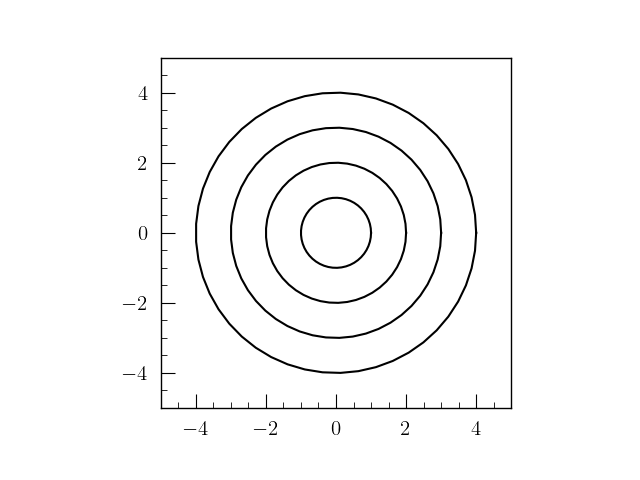
\includegraphics{./img/rotation.png}}
					\caption{$x^2 + y^2$一定.}
			    \end{minipage} &
			    \begin{minipage}{0.45\textwidth}
			    	\centering
					\scalebox{0.5}{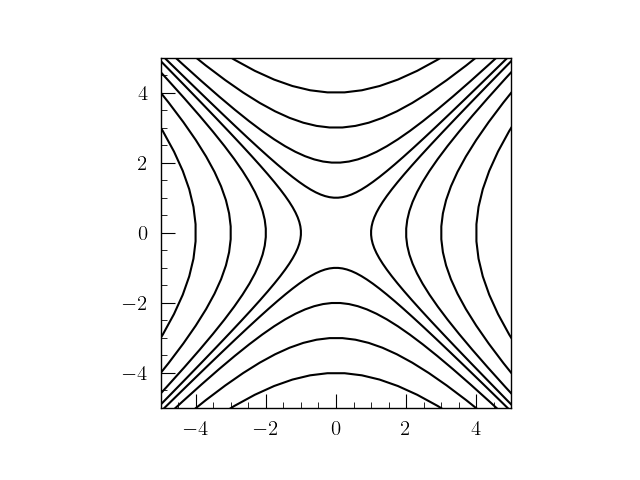
\includegraphics{./img/boost.png}}
					\caption{$t^2 - x^2$一定.}
			    \end{minipage}\\
					 & \\\hline
				$x' + y' = e^{i\theta}(x + y) $ & $t' + x' = e^{\eta}(t+x) $\\
				$x' - y' = e^{-i\theta}(x-y) $ & $t'-x' = e^{-\eta}(t-x)$\\\hline
				三角関数$\sin $, $\cos $ & 双曲線関数$\sinh $, $\cosh $\\\hline

		\end{tabular}
		\label{tab:trig_hypo}
\end{table}

		特殊相対論には(数学的には)Euclid幾何以上に不思議なことはなにもない.\footnote{$i$を使わない分マシとも言える.}
